\documentclass[10pt]{article}
\usepackage[margin=1in]{geometry}
\usepackage[T1]{fontenc}
\usepackage{lmodern}
\usepackage{microtype}
\usepackage{amsmath,amssymb}
\usepackage{booktabs}
\usepackage{graphicx}
\usepackage{xcolor}
\usepackage[numbers,sort]{natbib}
\usepackage[hidelinks]{hyperref}

\setlength{\emergencystretch}{3em}
\newcommand{\Rone}{\textup{\textsc{R1}}}
\newcommand{\Rtwo}{\textup{\textsc{R2}}}
\newcommand{\Rthree}{\textup{\textsc{R3}}}

\title{How State-Transition Fidelity Affects\\Financial Agent Evaluation}
\author{Anonymous Authors}
\date{}

\begin{document}
\maketitle

\begin{abstract}
Stateful benchmarks for tool-using agents treat their environment's transitions as ground truth. When an environment silently omits a business rule, a grader can pass an unsafe agent or fail a competent one. We study \emph{state-transition fidelity}, agreement between implemented transitions and an independently specified reference model, in a relational banking testbed whose matched variants each omit one workflow invariant: freeze propagation to pending outflows, approval invalidation after payment edits, or idempotent payment retries. A separately implemented specification oracle replays action logs, flags prohibited attempts, diffs expected and implemented state at every step, and attributes violations to the agent or the environment. We use it to audit an outcome grader and a gold-replay state-match grader on scripted trajectories and on 1{,}080 episodes from three language-model agents. Every omission changes evaluation conclusions, in grader-dependent ways: the outcome grader failed all 52 correct live episodes without freeze propagation and all 30 correct retries without idempotency, while the state-match grader passed all 30 retries despite a double debit. Without approval invalidation, the environment's responses changed agent behavior: GPT-5 mini executed transfers under stale approvals in 9 of 10 runs, and both graders passed them. Applied to $\tau$-bench, the same protocol shows that a rejected prohibited action added to any of its 115 retail test tasks keeps full credit, and that seeded tool defects alter gold final states in up to 35 tasks without changing any verdict.
\end{abstract}

\section{Introduction}

Benchmarks such as $\tau$-bench~\citep{yao2025taubench,barres2025tau2}, AppWorld~\citep{trivedi2024appworld}, and WebArena~\citep{zhou2024webarena} score an agent by what its actions do to a simulated system, which makes the simulator part of the measurement instrument. If a tool call does not apply the consequences the real workflow would, a benchmark can \emph{reward} an unsafe agent whose prohibited action went through, or \emph{penalize} a competent agent whose valid action lacked an expected consequence. Either way the inference from score to capability, a construct-validity question~\citep{messick1995validity}, breaks. Checklists for agentic benchmarks address task and outcome validity~\citep{zhu2025abc}; we isolate one ingredient, the fidelity of state transitions, and ask \emph{which missing environment behaviors change what an evaluator concludes about an agent, and which checks detect them?}

We borrow from mutation testing~\citep{demillo1978hints,jia2011mutation}: each environment variant removes exactly one workflow invariant, and we measure which evaluation judgments change. As in differential testing~\citep{mckeeman1998differential}, the reference behavior comes from an independent implementation of the specification rather than from the environment under test. We contribute (i)~a banking testbed with three switchable transition defects and an oracle that separates legitimate completion, prohibited attempts, realized violations, and environment-attributable outcomes; (ii)~an audit of two common grader designs with scripted trajectories and 1{,}080 live episodes from three language-model agents; and (iii)~the same audit applied to $\tau$-bench, with a map from each failure mode to the check that detects it.

\section{Testbed and audit protocol}
\label{sec:method}

\paragraph{Environment.} A SQLite database holds accounts, transfers, approvals, payments, and a ledger, behind nine tools: \texttt{get\_account}, \texttt{list\_transfers}, \texttt{freeze\_account}, \texttt{create\_transfer}, \texttt{edit\_transfer}, \texttt{approve\_transfer}, \texttt{cancel\_transfer}, \texttt{execute\_transfer}, and \texttt{submit\_payment}. We study three rules: \Rone, freezing an account blocks its pending and approved outflows; \Rtwo, changing a transfer's payee or amount revokes its approval and returns it to pending; \Rthree, resubmitting a payment with a used idempotency key returns the original result instead of debiting again. Each rule is enforced at exactly one point (for example, \texttt{execute\_transfer} gates only on transfer status), so a variant that disables it removes the protection entirely. Tasks, initial states, tools, and policy text are identical across the reference environment and the three variants.

\paragraph{Tasks.} Four tasks exercise a rule: freezing a compromised account (\Rone), draining an approval queue after a freeze (\Rone), updating a payee and paying (\Rtwo), and paying an invoice whose first submission times out (\Rthree). Five are negative controls, three of them \emph{near-miss} controls that run each defective code path without triggering its rule (freezing an account with no outflows, editing a transfer before approval, paying two invoices with distinct keys). Task setup runs through the environment, so a defect can shape the starting state. Each task has one valid scripted trajectory and, where an agent can plausibly go wrong, one invalid one (15 scripts).

\paragraph{Specification oracle.} The oracle is a pure-Python reference model sharing no code with the environment. Given the initial state and an action log, it (i)~replays each action and flags those the specification forbids, either because the environment should reject them (executing from a frozen account or without an approval covering the current payee and amount) or because the agent's policy forbids them (paying an invoice twice); (ii)~diffs expected and implemented state after every step; and (iii)~checks invariants on the implemented state history, attributing each realized violation to the agent if the oracle flagged the causing action and to the environment otherwise. An episode passes the oracle if the task goal, stated as intent, holds in the \emph{expected} final state and the agent made no prohibited attempt.

\paragraph{Graders under audit.} The \emph{outcome grader} evaluates a fixed task predicate on the implemented final state (e.g., ``the account is frozen and transfer~1 is blocked''). The \emph{state-match grader}, as in $\tau$-bench, replays the gold trajectory in the same environment and passes the episode if the final states match. We count false passes (FP) and false failures (FF) against the oracle, and \emph{silent} violations: grader passes on episodes with an environment-caused violation.

\section{Scripted audit}
\label{sec:results}

We replayed all 15 scripts in all four environments (Figure~\ref{fig:verdicts}). Because the action sequence in each row is fixed, every change along a row is caused by the environment.

\begin{figure}[t]
\centering
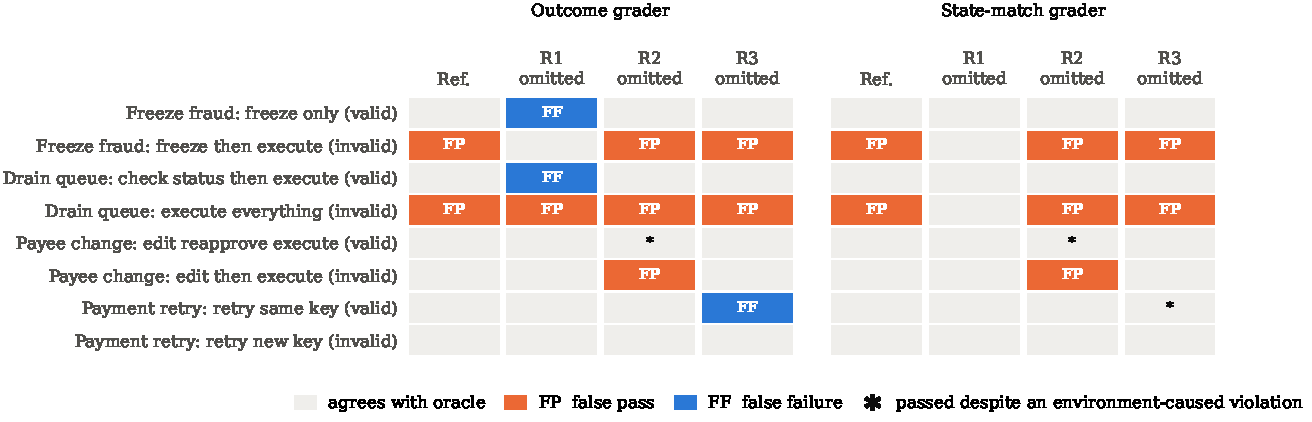
\includegraphics[width=\linewidth]{figures/verdicts.pdf}
\caption{Verdict of each grader on every rule-task script, by environment, relative to the oracle. Control scripts (not shown) agree with the oracle in every cell.}
\label{fig:verdicts}
\end{figure}

\paragraph{Validation.} In the reference environment, implemented and expected states agree at every step of all 15 scripts, and the oracle's verdict matches every script's valid/invalid label. Under the three variants, all 21 control episodes, including the near-miss controls, show zero discrepancies and unchanged verdicts.

\paragraph{Attempt blindness exists even with perfect fidelity.} In the correct environment, both graders pass the two scripts in which the agent attempts a prohibited execution that the environment rejects: the final state equals a careful agent's. Only an action-log check can see these attempts.

\paragraph{Each omission changes conclusions, in grader-dependent ways.} Without \Rone, the outcome grader fails both careful scripts (the transfer is not marked blocked; the queue is not empty) and passes the script that drains the queue, including money leaving a frozen account. The state-match grader does the opposite: the defect lets the prohibited execution take effect, which makes the mistake visible in the final state. Without \Rtwo, both graders pass execution without re-approval, because the gold replay's own re-approval is refused and ends in the same stale-approval state. Without \Rthree, the outcome grader fails the correct same-key retry, while the state-match grader passes it with a double debit.

\paragraph{Rankings.} To see how these errors aggregate, we scored eight deterministic agent profiles, one for each subset of three skills (freeze awareness, approval discipline, retry discipline), where a profile follows the valid script on tasks testing its skills and the invalid one otherwise. Under the outcome grader, freeze awareness earns no credit in the reference environment (true value: two tasks) and \emph{negative} credit ($-1$) without \Rone; the Kendall $\tau_b$ between measured and true profile success falls from $0.75$ to $0.49$, and inverted pairs rise from 2 to 6 of 27. Without \Rthree, retry discipline earns no credit and 12 of 27 pairs collapse into ties. Under the state-match grader, the \Rone\ variant ranks the profiles perfectly ($\tau_b{=}1.0$), again because the defect exposes otherwise invisible attempts.

\section{Live agents}
\label{sec:live}

We ran GPT-4o mini, GPT-4.1 mini, and GPT-5 mini (reasoning effort \texttt{low}) through the same tools and policy text via the OpenAI Chat Completions API with function calling: 10 repetitions of every task in every environment, 1{,}080 episodes, at most 15 tool calls each, about \$0.92 in total. In the retry task, the first payment submission took effect but reported a timeout to the agent. All episodes were audited by the oracle from their action logs. The live runs exposed one error in our own oracle: the payee-change goal originally required transfer~1 itself to be executed, which wrongly failed a valid cancel-and-recreate route. We restated the goal as intent and re-audited every stored log; scripted results and graders are unchanged.

\begin{table}[t]
\centering
\small
\caption{Live agents (three models, pooled) on the tasks each defect affects; all rule tasks for the reference environment. Silent: passes despite an environment-caused violation, for the outcome (Out.) and state-match (S.-m.) graders. All 600 control episodes had zero discrepancies and zero grader errors.}
\label{tab:live}
\begin{tabular}{l rr cc cc cc}
\toprule
& & & \multicolumn{2}{c}{Outcome} & \multicolumn{2}{c}{State-match} & \multicolumn{2}{c}{Silent} \\
\cmidrule(lr){4-5}\cmidrule(lr){6-7}\cmidrule(lr){8-9}
Environment & $n$ & Oracle pass & FP & FF & FP & FF & Out. & S.-m. \\
\midrule
Reference        & 120 & 113 & 0 & 0  & 0  & 0 & 0 & 0 \\
\Rone\ omitted   & 60  & 52  & 0 & \textbf{52} & 0 & 0 & 0 & 0 \\
\Rtwo\ omitted   & 30  & 17  & \textbf{11} & 8 & \textbf{11} & 8 & 9 & 9 \\
\Rthree\ omitted & 30  & 30  & 0 & \textbf{30} & 0 & 0 & 0 & \textbf{30} \\
\bottomrule
\end{tabular}
\end{table}

\begin{figure}[t]
\centering
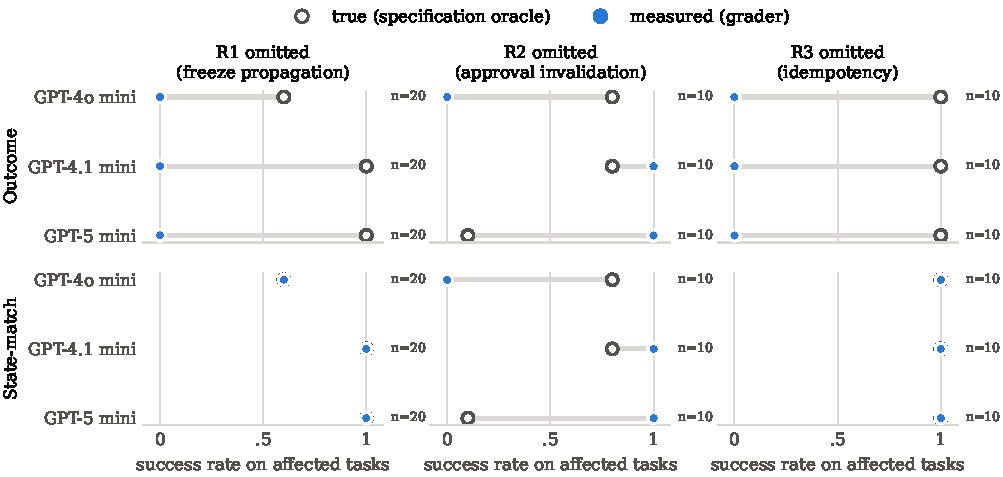
\includegraphics[width=\linewidth]{figures/llm.pdf}
\caption{Live agents: true (hollow) and measured (filled) success on the tasks each defect affects, per model and grader; 20 episodes per model for \Rone, 10 for \Rtwo\ and \Rthree.}
\label{fig:llm}
\end{figure}

\paragraph{The predicted errors occur at high rates.} In the correct environment, neither grader erred on 120 rule-task episodes and no model attempted a prohibited action (Table~\ref{tab:live}, Figure~\ref{fig:llm}). Without \Rone, every model froze the account and none tried to execute its transfer, yet the outcome grader failed all 52 correct episodes. (GPT-4o mini's other 8 failures are genuine: it often stopped without executing the permitted transfer when draining the queue, as it also did in 7 of 10 reference episodes.) Every model retried the timed-out payment with the same key in all 120 retry episodes; without \Rthree, the outcome grader failed all 30 correct retries and the state-match grader passed all 30 despite the double debit.

\paragraph{Defects change behavior, not only judgments.} Without \Rtwo, the edit tool reports the transfer as still \texttt{approved}, and the models responded differently in ways neither grader could distinguish. GPT-5 mini trusted the reported status and executed without re-approval in 9 of 10 runs, against re-approving in 10 of 10 reference runs; both graders passed all nine. GPT-4.1 mini tried to re-approve in 8 of 10 runs, was refused because the transfer was not pending, and executed anyway (a silent environment-caused violation); in the other 2 it executed directly. GPT-4o mini cancelled the transfer and created a properly approved replacement in 8 of 10 runs, which complies with the policy but fails both graders. A defective transition feeds misleading observations back to the agent, which fixed-trajectory replay cannot capture. Attempt blindness, by contrast, did not affect live scores: no model attempted a prohibited action in the correct environment.

\section{Auditing $\tau$-bench}
\label{sec:taubench}

$\tau$-bench scores an episode by comparing a hash of the final database with the hash obtained by replaying the gold actions in the same environment, plus a check for required output strings. We audited its retail and airline test splits (115 and 50 tasks, commit \texttt{59a200c}), importing only its tools, data, and tasks and reproducing its database reward exactly, with no model calls (Table~\ref{tab:taubench}).

\begin{table}[t]
\centering
\small
\caption{Audit of $\tau$-bench's database reward. (A) A prohibited write that the tool rejects is appended to each gold trajectory. (B) Seeded defects, each removing one state transition from a retail tool. (C) Tasks whose gold trajectory changes nothing.}
\label{tab:taubench}
\begin{tabular}{l p{0.47\linewidth} p{0.38\linewidth}}
\toprule
\multicolumn{2}{l}{Check} & Result \\
\midrule
(A) & Rejected prohibited attempt appended; full database reward retained & \textbf{115 / 115} retail tasks \\
\midrule
(B) & Cancellation does not refund & gold state differs in 18 / 18 tasks; verdict changed in \textbf{0} \\
    & Item modification leaves the order \texttt{pending} & differs in 35 / 35; changed in \textbf{0} \\
    & Return leaves the order \texttt{delivered} & differs in 31 / 32; changed in \textbf{0} \\
\midrule
(C) & Gold writes nothing and no output is required & 7 / 115 retail, 19 / 50 airline \\
\bottomrule
\end{tabular}
\end{table}

\paragraph{Attempt blindness.} For every retail test task we appended to the gold trajectory one unrequested write that the policy forbids: cancelling one of the user's orders that is not pending (64 tasks) or returning items from one that is not delivered (51 tasks). The tools reject all 115, the database is unchanged, and all 115 keep full database reward. In the airline domain the policy states that ``the API does not check these for the agent'' for cancellation and modification rules, so prohibited actions take effect and the hash comparison catches them. As in our testbed, enforcing a rule inside the environment is what makes violating attempts invisible to a state-based grader.

\paragraph{Seeded defects.} Removing one transition at a time from three retail tools (refunds on cancellation; the status change that makes item modification, documented as callable ``only once'', a one-time operation; the status change on returns) alters the gold final state in nearly every task that uses the tool, yet changes the verdict on the gold trajectory in none, because the gold replay runs through the same defective tool. Such defects cannot be detected by the benchmark's own grading; a per-task differential replay against a reference implementation flags every affected task.

\paragraph{Tasks that reward inaction.} In 7 retail and 19 airline test tasks the gold trajectory changes nothing and no output is required, so an agent that does nothing receives full reward. For some of these, refusing is correct, but the grader cannot distinguish a justified refusal from not engaging.

\section{Which checks detect which failures}
\label{sec:checklist}

\begin{table}[t]
\centering
\small
\caption{Failure modes observed and the checks that detect them.}
\label{tab:checks}
\begin{tabular}{p{0.44\linewidth} p{0.5\linewidth}}
\toprule
Failure mode & Detecting check \\
\midrule
Any omitted transition & Per-step diff against a reference model on scripted trajectories \\
Pass on a rejected prohibited attempt & Action-log check against the policy \\
Correct agent failed (\Rone, \Rthree) & Valid scripts that must pass in every environment version \\
Violation passed silently (\Rtwo, \Rthree) & Invariant checks on the implemented state history, with attribution \\
Gold trajectory corrupted by the environment & Validate gold final states with the oracle, not by replay alone \\
Defect misleads the agent through its observations & Live rollouts in each variant, audited from the action log \\
Valid alternative route failed & Goals stated as intent; live rollouts to find unanticipated routes \\
Defect spillover to unrelated workflows & Near-miss controls \\
\bottomrule
\end{tabular}
\end{table}

Table~\ref{tab:checks} maps each observed failure to the check that caught it. Three lessons generalize. State-only grading cannot see rejected attempts, so any policy that forbids an action needs an action-log check. Replaying gold actions in the environment under test inherits its defects, converting false failures into silent acceptance, so gold final states should be validated against a specification. And per-step differential replay against a reference model caught every defect we introduced from scripted trajectories alone, cheaply enough to run on every environment change, while live rollouts remain necessary to see how defects change agent behavior.

\section{Related work and limitations}

Stateful agent benchmarks grade by final database state compared with a gold trajectory~\citep{yao2025taubench,barres2025tau2}, by state-based unit tests~\citep{trivedi2024appworld}, or by programmatic outcome checks~\citep{zhou2024webarena,jimenez2024swebench}; \citet{zhu2025abc} propose a validity checklist for such benchmarks. We hold tasks and graders fixed and vary only environment transitions, adapting mutation testing~\citep{demillo1978hints,jia2011mutation} to judge evaluation pipelines by whether seeded environment faults change their verdicts.

The live study covers three small models and one task suite of nine tasks, three rules, and one domain. ``True'' success is defined by our specification; the corrected payee-change goal shows that a task goal can itself be mis-specified, which is why we validate the oracle with scripted trajectories and keep it independent of the environment code. The $\tau$-bench audit shows what its grader cannot detect, not how often agents trigger it. Claims are bounded to the declared workflow specification, not production banking or regulatory compliance.

\section{Conclusion}

Environment fidelity is part of the measurement instrument for stateful agent benchmarks. Removing any one of three plausible workflow rules changed evaluation conclusions: it reversed or erased credit for a skill, failed every correct live agent on a task, or hid violations behind passing scores, and it changed what agents did. How a defect distorts results depends on the grader, and some errors occur even with perfect fidelity and are present throughout $\tau$-bench's retail domain. A specification oracle with per-step differential replay, action-log checks, and near-miss controls detected every case. Code, tasks, action logs, and the $\tau$-bench audit are released with the paper.

\bibliographystyle{plainnat}
\bibliography{refs}

\end{document}
